\section{Test}

\subsection{Specifica dei test}

Per garantire la qualità del prodotto, Three Way Milkshake adotta il modello a V\textsubscript{G} per verificare tramite test ogni passo della produzione software.\\Qui vedremo un'immagine rappresentativa del modello a V\textsubscript{G} (o V-Model), quest'ultimo si può schematizzare posizionando il tempo nell'asse delle ascisse e il livello di astrazione nell'asse delle ordinate.\\Il modello idealmente si divide in 2 rami.\\Il ramo sinistro contiene le fasi\textsubscript{G} di progettazione e ideazione; il ramo destro contiene le fasi\textsubscript{G} di test e integrazione.
\begin{figure}[h!]
	\centering
	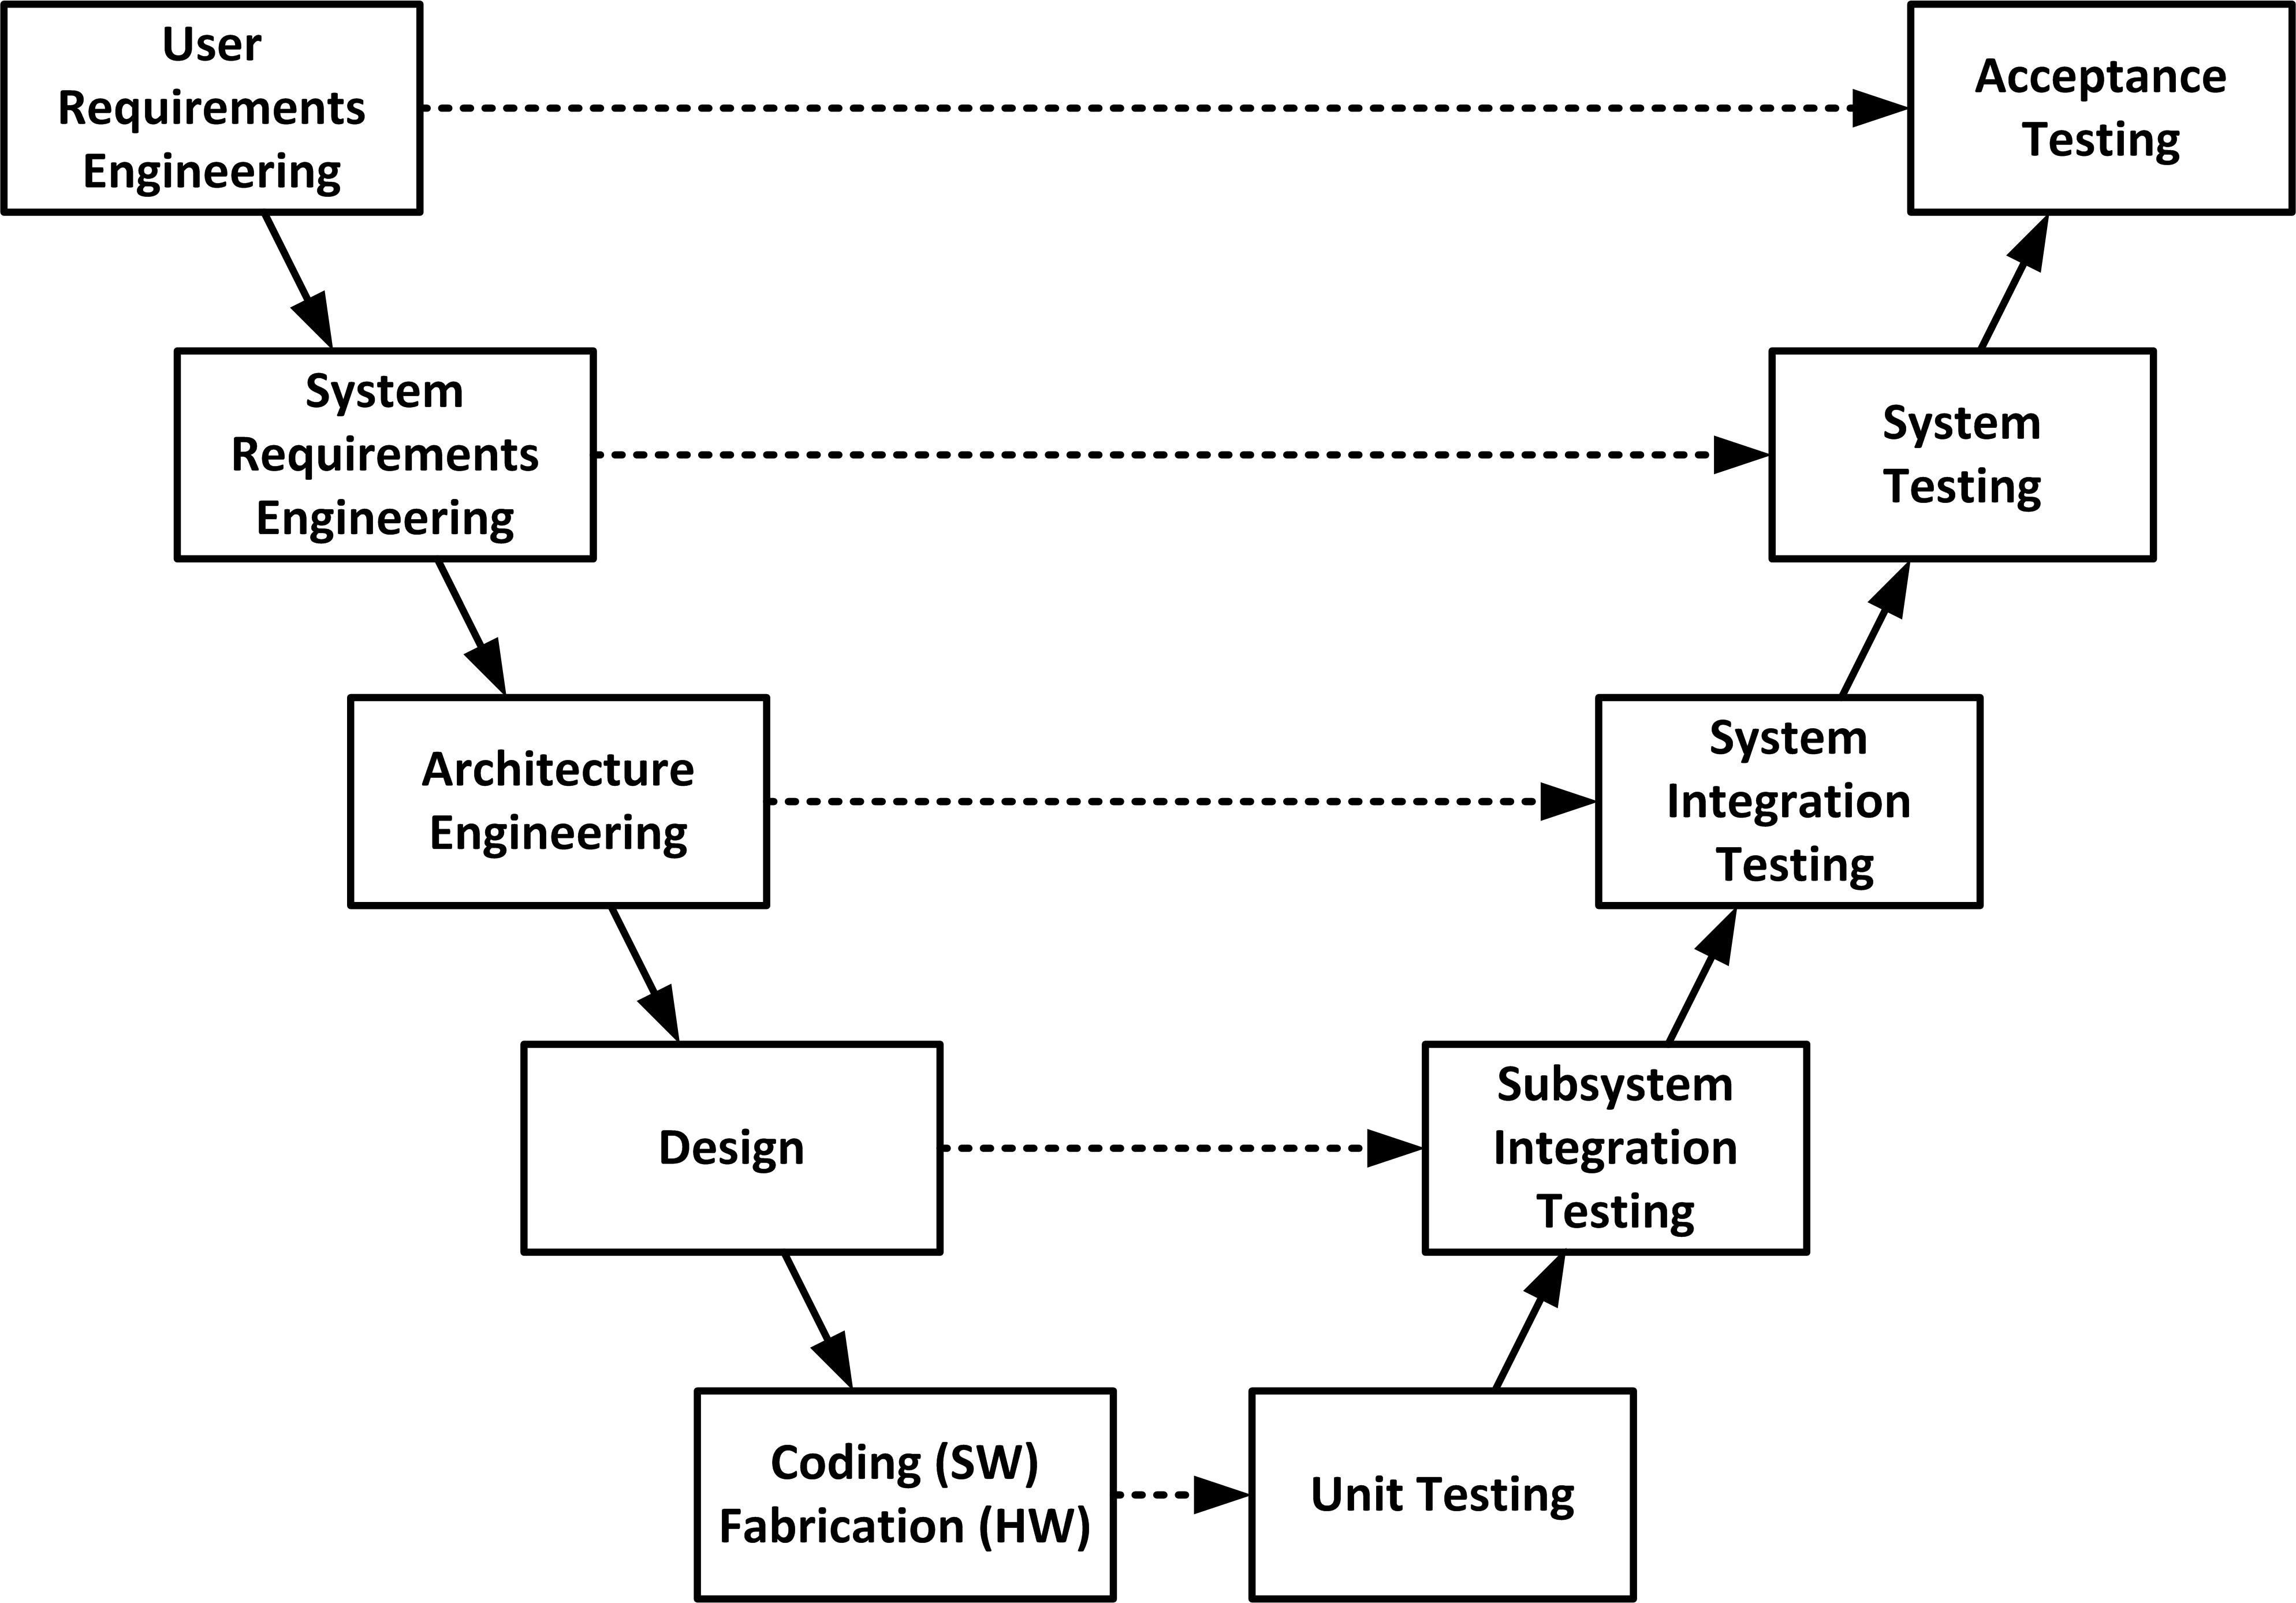
\includegraphics[scale=0.6]{res/images/v_model.jpg}
	\caption{Figura esplicativa del {modello a V}}
\end{figure}
\newline
Per definire lo stato dei test viene utilizzato un valore da 0 a 2:
\begin{itemize}
	\item \textbf{0:} il test non è stato implementato;
	\item \textbf{1:} il test è stato implementato, ma fallisce;
	\item \textbf{2:} il test è stato implementato e superato.
\end{itemize}
Vi sono quattro tipi di test:
\begin{itemize}
	\item accettazione;
	\item sistema;
	\item integrazione;
	\item unità.
\end{itemize}

\subsection{Test di Accettazione}
Verificano che il software nel suo complesso soddisfi i criteri di accettazione decisi con il cliente, verranno indicati nel seguente modo:\\
\begin{center}
	TA[Codice]-[Importanza]\\
\end{center}
dove:
\begin{itemize}
	\item \textbf{Codice:} rappresenta il codice identificativo crescente del componente da verificare.
	\item \textbf{Importanza:} indica l'importanza del requisito\textsubscript{G} che può essere:
		\begin{itemize}
			\item \textbf{O} per i requisiti\textsubscript{G} obbligatori;
			\item \textbf{D} per i requisiti\textsubscript{G} desiderabili;
			\item \textbf{F} per i requisiti\textsubscript{G} facoltativi.
		\end{itemize}
\end{itemize}

%tabella
	\begin{longtable}{ >{\centering}p{0.20\textwidth} >{}p{0.75\textwidth}}


	\caption{Riepilogo Test di Accettazione}\\
	\hline
	\rowcolorhead
	\headertitle{Requisito} & \headertitle{Descrizione}
	\endfirsthead
	\caption[]{(continua)}\\
	\rowcolorhead
	\headertitle{Requisito} & \headertitle{Descrizione}
	\endhead



	TA1-O & L'utente deve poter fare il login alla piattaforma, tramite codice identificativo e password. \tabularnewline

	TA1.1-O & Se il codice e/o la password non sono corretti o non esistono nel sistema \newline il login fallisce.\tabularnewline

	TA2-O & L'amministratore deve poter registrare un nuovo account di un responsabile. \tabularnewline

	%% TAF-2.1-O & In caso di registrazione fallita (per lavoratore già esistente); allora deve venir mostrato un messaggio d'errore.\tabularnewline

	TA3-O & L'amministratore può gestire un account già esistente,in particolare modificarne nome, cognome e password.\tabularnewline
	TA3.1-O & L'amministratore può eliminare un account già esistente.\tabularnewline
	TA3.2-O & L'amministratore può richiedere il reset password di un preciso account.\tabularnewline
	TA3.3-O & L'amministratore può visualizzare una lista di tutti gli utenti registrati con i loro dati pubblici. \tabularnewline

	TA4-O & Il responsabile deve poter aggiungere una task\textsubscript{G} alla lista delle task\textsubscript{G}. \tabularnewline


	%%TAF-5-O & Il responsabile deve poter modificare la priorità di una task\textsubscript{G}.\newline Al responsabile è richiesto di: \begin{itemize}\item autenticarsi con il suo account; \item selezionare la task\textsubscript{G} da modificare; \item inserire la nuova priorità; \item confermare la modifica priorità della task\textsubscript{G}. \end{itemize}\tabularnewline

	TA5-O & Il responsabile deve poter eliminare una task\textsubscript{G} dalla lista delle task\textsubscript{G}. \tabularnewline

	TA6-O & Il sistema deve permettere all'amministratore e al responsabile di effettuare il logout dall'applicativo.\tabularnewline
	TA6.1-O & Il sistema deve permettere a responsabile e amministratore di effettuare il logout in qualsiasi momento. \tabularnewline

	TA7-O & Il sistema deve permettere a responsabili e amministratore di visualizzare la mappa, e in particolare visualizzare i POI\textsubscript{A}, aree non transitabili, muletti in real-time e le zone di percorrenza\textsubscript{G}. \tabularnewline

	TA8-O & Il sistema deve permettere all'amministratore la visualizzazione di una notifica in caso della segnalazione da parte di un utente di un evento eccezionale.\tabularnewline

	TA8.1-F & Il sistema deve permettere agli utenti la visualizzazione delle persone in real-time sulla mappa\tabularnewline
	
	TA8.2-O & Il sistema deve permettere la visualizzazione di direzione e spostamento del muletto a cui è a bordo. \tabularnewline
	
	TA8.3-O & Il sistema deve permettere la visualizzazione del prossimo POI\textsubscript{A} da raggiungre con un colore diverso. \tabularnewline

	TA9-O & Il sistema deve permettere all'amministratore di modificare la mappa, in particolare modificare planimetria\textsubscript{G} e percorrenza\textsubscript{G}. \tabularnewline
	TA9.1-O & Il sistema deve permettere all'amministratore di gestire i POI\textsubscript{A} nella mappa, in particolare modificarne la posizione di uno già esistente. \tabularnewline
	TA9.2-O & Il sistema deve permettere all'amministratore di eliminare un POI\textsubscript{A} già esistente. \tabularnewline
	TA9.3-O & Il sistema deve permettere all'amministratore di creare un nuovo POI\textsubscript{A}. \tabularnewline

	TA10-O & L'operatore deve poter accedere alla sua user interface.\tabularnewline

	TA10.1-O & L'operatore deve poter vedere sotto alla mappa una lista ordinata delle task\textsubscript{G} rimanenti da eseguire dall'operatore.\newline Nella user interface dell'operatore, sotto la mappa deve apparire una lista ordinata contenente le task\textsubscript{G} rimanenti da soddisfare.\tabularnewline
	TA10.2-O & L'operatore deve poter vedere nella mappa il prossimo task\textsubscript{G} da soddisfare(POI\textsubscript{A} da raggiungere) (evidenziato con colore diverso).\newline Nella user interface dell'operatore, nella mappa deve mostrare il prossimo task\textsubscript{G} da raggiungere.\tabularnewline
	TA10.3-O & L'operatore deve poter segnalare la conclusione dell'incarico attraverso la user interface.\newline Nella propria user interface, l'operatore deve cliccare sul POI\textsubscript{A} evidenziato (raggiunto) nella mappa e confermare l'avvenuto scarico.\tabularnewline
	TA10.4-O & L'operatore deve poter vedere direzione e spostamento del muletto a cui è a bordo, in caso sia attiva la guida automatica; in particolare il sistema deve attivare le icone di frecce direzionali, start e stop. \tabularnewline
	TA10.5-O & L'operatore deve poter passare da guida manuale a guida automatica attraverso la user interface, premendo l'apposito pulsante per cambiare tipo di guida (manuale, automatica).\tabularnewline
	TA10.6-O & L'operatore deve poter segnalare un evento eccezionale al server attraverso la user interface.\newline All'utente è richiesto di segnalare un evento eccezionale, attraverso l'apposito pulsante.\tabularnewline
	TA10.7-O & L'operatore deve poter impostare la guida automatica verso la base, dopo aver finito tutte le task\textsubscript{G}, attraverso l'apposito pulsante nella user interface.\tabularnewline
	TA10.8-O & La user interface che rappresenta una singola unità, deve prevedere pulsanti per 4 frecce direzionali, start e stop per gli spostamenti manuali.\tabularnewline

	TA11-D & Il pannello permette di visualizzare l'indicatore di velocità attuale.\tabularnewline

	TA12-O & Il sistema centrale deve pilotare e coordinare tutte le unità per evitare ingorghi e incidenti.\tabularnewline
	TA12.1-F & Il sistema fornisce il percorso migliore alle unità tramite algoritmi di ricerca operativa.\tabularnewline

	TA13-O & Il sistema deve permettere a amministratore e responsabili di visualizzare la lista di tutti i POI\textsubscript{A} presenti nella mappa.\tabularnewline

	TA14-O & Il responsabile deve poter vedere tutte le liste ordinate di task\textsubscript{G}, divise per liste non ancora prese in carico da un'unità e quelle già assegnate. \tabularnewline

	TA15-O & L'amministratore deve poter accedere a un'interfaccia per aggiungere o rimuovere un'unità. \tabularnewline
	
	TA15.1-O & L'amministratore deve poter aggiungere un'unità. \tabularnewline

	TA15.2-O & L'amministratore deve poter rimuovere un'unità. \tabularnewline

	TA15.3-O & Il server centrale deve poter conoscere la posizione nella mappa di una precisa unità (e quindi potenzialmente di tutte).\tabularnewline
	TA15.4-O & Il server centrale deve poter inviare il percorso che l'unità deve fare per spostarsi da un POI\textsubscript{A} al prossimo.\tabularnewline

	TA16-O & La geo localizzazione va simulata.\tabularnewline
	TA16.1-O & L'applicativo propone una mappatura in tempo reale della posizione geo referenziata delle unità.\tabularnewline
	TA16-2-F & L'applicativo propone una mappatura in tempo reale della posizione geo referenziata delle persone.\tabularnewline

	TA17-O & Il server centrale deve poter prevedere ed evitare le collisioni.\tabularnewline
	TA17.1-O & Ogni unità deve rispettare i vincoli dimensionali delle zone.\tabularnewline
	TA17.2-O & Tutte le unità in movimento devono viaggiare alla stessa velocità, che rimane costante.\tabularnewline
	TA17.3-O & Ogni unità ha una velocità massima, velocità di crociera e codice identificativo.	\tabularnewline
	TA17.4-F & Il server centrale permette di gestire il cambiamento di velocità di un'unità.\tabularnewline

	TA18-O & Il server centrale conosce la posizione/direzione/velocità di ogni singola unità. \tabularnewline

	TA19-O & Ogni task\textsubscript{G} è collegata ad un POI\textsubscript{A} da raggiungere.\tabularnewline
	TA19.1-O & Ogni POI\textsubscript{A} può essere di carico, scarico o base.\tabularnewline
	TA19.2-O & Ci devono essere almeno un POI\textsubscript{A} di carico e di base, e più di un POI\textsubscript{A} di scarico. \tabularnewline

	TA20-O & Ogni unità parte da una base (inizio turno operatore) e torna ad una base, quando finisce il turno dell'operatore.\tabularnewline
	TA20.1-O & Ogni unità passa per un'area di carico prima di iniziare la sequenza di scarichi (tasks).\tabularnewline
	TA20.2-O & Ogni unità torna ad un'area di carico se ha completato i task\textsubscript{G} e il turno dell'operatore non è terminato.\tabularnewline
	TA21-O & Il server centrale conosce ogni spostamento, partenza e fermata di ogni singola unità.\tabularnewline
	TA22-O & Ci deve essere uno e un solo account registrato con ruolo amministratore.\tabularnewline
	TA22.1-O & Ci deve essere almeno un account con ruolo responsabile.\tabularnewline
	TA22.2-O & Ci possono essere più account con ruolo responsabile.\tabularnewline



\end{longtable}
%fine tabella
\pagebreak
\subsection{Test di Sistema}
I Test di Sistema verificano la conformità dell'intero sistema con i requisiti\textsubscript{G} specificati.\\I Test di Sistema verranno sviluppati quando verrà raggiunto il macro periodo\textsubscript{G} appropriata, secondo il modello a V\textsubscript{G}.
\begin{center}
	TS[Codice]-[Importanza]\\
\end{center}
dove:
\begin{itemize}
	\item \textbf{Codice:} rappresenta il codice identificativo crescente del componente da verificare.
	\item \textbf{Importanza:} indica l'importanza del requisito\textsubscript{G} che può essere:
	\begin{itemize}
		\item \textbf{O} per i requisiti\textsubscript{G} obbligatori;
		\item \textbf{D} per i requisiti\textsubscript{G} desiderabili;
		\item \textbf{F} per i requisiti\textsubscript{G} facoltativi.
	\end{itemize}
\end{itemize}


	\begin{longtable}{ >{\centering}p{0.20\textwidth} >{}p{0.75\textwidth}}
	
	
	\caption{Riepilogo Test di Sistema}\\
	\hline
	\rowcolorhead
	\headertitle{Requisito} & \headertitle{Descrizione}
	\endfirsthead
	\caption[]{(continua)}\\
	\rowcolorhead
	\headertitle{Requisito} & \headertitle{Descrizione}
	\endhead
	
	
	
	TS1-O & L'utente deve poter fare il login.\newline All'utente viene chiesto di: \begin{itemize}\item accedere alla pagina di login;\item inserire il proprio codice identificativo;\item inserire la password.\end{itemize}\tabularnewline
	
	TS1.1-O & Se il codice e/o la password non sono corretti o non esistono nel sistema \newline il login fallisce.\newline Se il login dell'utente non va a buon fine deve venir mostrato un messaggio d'errore.\tabularnewline
	
	TS2-O & L'amministratore deve poter registrare un nuovo account di un responsabile.\newline All'amministratore viene chiesto di: \begin{itemize}\item inserire nome; \item inserire cognome.\end{itemize}\tabularnewline
	
	%% TAF-2.1-O & In caso di registrazione fallita (per lavoratore già esistente); allora deve venir mostrato un messaggio d'errore.\tabularnewline
	
	TS3-O & L'amministratore può gestire un account già esistente.\newline In particolare può: \begin{itemize}\item modificare campo nome; \item modificare campo cognome; \item modificare password. \end{itemize}\tabularnewline
	TS3.1-O & L'amministratore può eliminare un account già esistente.\tabularnewline
	TS3.2-O & L'amministratore può richiedere il reset password di un preciso account.\tabularnewline
	TS3.3-O & L'amministratore può visualizzare una lista di tutti gli utenti registrati con i loro dati pubblici. \tabularnewline
	
	TS4-O & Il responsabile deve poter aggiungere una task\textsubscript{G} alla lista delle task\textsubscript{G}.\newline Al responsabile è richiesto di: \begin{itemize}\item autenticarsi con account con ruolo responsabile; \item selezionare il pulsante per aggiungere una nuova task\textsubscript{G}; \item inserire il POI\textsubscript{A} a cui fa riferimento; \item confermare l'inserimento di nuova task\textsubscript{G}. \end{itemize}\tabularnewline
	
	
	%%TAF-5-O & Il responsabile deve poter modificare la priorità di una task\textsubscript{G}.\newline Al responsabile è richiesto di: \begin{itemize}\item autenticarsi con il suo account; \item selezionare la task\textsubscript{G} da modificare; \item inserire la nuova priorità; \item confermare la modifica priorità della task\textsubscript{G}. \end{itemize}\tabularnewline
	
	TS5-O & Il responsabile deve poter eliminare una task\textsubscript{G} dalla lista delle task\textsubscript{G}.\newline Al responsabile è richiesto di: \begin{itemize} \item autenticarsi con il suo account; \item selezionare la task\textsubscript{G} da eliminare; \item confermare l'eliminazione della task\textsubscript{G}. \end{itemize}\tabularnewline
	
	TS6-O & Il sistema deve permettere all'amministratore e al responsabile di effettuare il logout dall'applicativo.\tabularnewline
	TS6.1-O & Il sistema deve permettere a responsabile e amministratore di effettuare il logout in qualsiasi momento.\newline Al responsabile/amministratore è richiesto di: \begin{itemize} \item premere il pulsante logout nell'applicativo. \end{itemize}\tabularnewline
	
	TS7-O & Il sistema deve permettere a responsabili e amministratore di visualizzare la mappa, e in particolare visualizzare i POI\textsubscript{A}, aree non transitabili, muletti in real-time e le zone di percorrenza\textsubscript{G}.\newline All'utente è richiesto:\begin{itemize} \item autenticarsi come responsabile o amministratore; \item selezionare il pulsante per la visualizzazione della mappa; \item visualizzare i vari elementi della mappa (POI\textsubscript{A}, zona di percorrenza\textsubscript{G}, aree non transitabili e muletti in real-time). \end{itemize}\tabularnewline
	
	TS8-O & Il sistema deve permettere all'amministratore la visualizzazione di una notifica in caso della segnalazione da parte di un utente di un evento eccezionale.\tabularnewline
	
	TS8.1-F & Il sistema deve permettere agli utenti la visualizzazione delle persone in real-time sulla mappa\tabularnewline
	
	TS8.2-O & Il sistema deve permettere la visualizzazione di direzione e spostamento del muletto a cui è a bordo. \tabularnewline
	
	TS8.3-O & Il sistema deve permettere la visualizzazione del prossimo POI\textsubscript{A} da raggiungre con un colore diverso. \tabularnewline
	
	TS9-O & Il sistema deve permettere all'amministratore di modificare la mappa, in particolare modificare planimetria\textsubscript{G} e percorrenza\textsubscript{G}.\newline All'utente è richiesto: \begin{itemize} \item autenticarsi come amministratore; \item selezionare il pulsante per la gestione mappa; \item selezionare il pulsante relativo alla modifica della mappa da effettuare.\end{itemize}\tabularnewline
	TS9.1-O & Il sistema deve permettere all'amministratore di gestire i POI\textsubscript{A} nella mappa, in particolare modificarne la posizione di uno già esistente.\newline All'amministratore è richiesto: \begin{itemize}\item autenticarsi come amministratore; \item selezionare il pulsante per la gestione mappa; \item selezionare il pulsante per la gestione dei POI\textsubscript{A}; \item selezionare il pulsante per la modifica della posizione di un POI\textsubscript{A}; \item selezionare il POI\textsubscript{A} interessato e aggiornarne la posizione.\end{itemize}\tabularnewline
	TS9.2-O & Il sistema deve permettere all'amministratore di eliminare un POI\textsubscript{A} già esistente.\newline All'amministratore è richiesto: \begin{itemize}\item autenticarsi come amministratore; \item selezionare il pulsante per la gestione mappa; \item selezionare il pulsante per la gestione dei POI\textsubscript{A}; \item selezionare il POI\textsubscript{A} da eliminare; \item selezionare il pulsante di eliminazione del POI\textsubscript{A}.\end{itemize}\tabularnewline
	TS9.3-O & Il sistema deve permettere all'amministratore di creare un nuovo POI\textsubscript{A}.\newline All'amministratore è richiesto: \begin{itemize}\item autenticarsi come amministratore; \item selezionare il pulsante per la gestione mappa; \item inserire codice identificativo, posizione nella mappa, tipo di POI\textsubscript{A} (carico, scarico, base) del nuovo POI\textsubscript{A}; \item selezionare il pulsante di conferma dell'aggiunta del POI\textsubscript{A}.\end{itemize}\tabularnewline
	
	TS10-O & L'operatore deve poter accedere alla sua user interface.\tabularnewline
	
	TS10.1-O & L'operatore deve poter vedere sotto alla mappa una lista ordinata delle task\textsubscript{G} rimanenti da eseguire dall'operatore.\newline Nella user interface dell'operatore, sotto la mappa deve apparire una lista ordinata contenente le task\textsubscript{G} rimanenti da soddisfare.\tabularnewline
	TS10.2-O & L'operatore deve poter vedere nella mappa il prossimo task\textsubscript{G} da soddisfare(POI\textsubscript{A} da raggiungere) (evidenziato con colore diverso).\newline Nella user interface dell'operatore, nella mappa deve mostrare il prossimo task\textsubscript{G} da raggiungere.\tabularnewline
	TS10.3-O & L'operatore deve poter segnalare la conclusione dell'incarico attraverso la user interface.\newline Nella propria user interface, l'operatore deve cliccare sul POI\textsubscript{A} evidenziato (raggiunto) nella mappa e confermare l'avvenuto scarico.\tabularnewline
	TS10.4-O & L'operatore deve poter vedere direzione e spostamento del muletto a cui è a bordo, in caso sia attiva la guida automatica; in particolare il sistema deve attivare le icone di frecce direzionali, start e stop. \tabularnewline
	TS10.5-O & L'operatore deve poter passare da guida manuale a guida automatica attraverso la user interface, premendo l'apposito pulsante per cambiare tipo di guida (manuale, automatica).\tabularnewline
	TS10.6-O & L'operatore deve poter segnalare un evento eccezionale al server attraverso la user interface.\newline All'utente è richiesto di segnalare un evento eccezionale, attraverso l'apposito pulsante.\tabularnewline
	TS10.7-O & L'operatore deve poter impostare la guida automatica verso la base, dopo aver finito tutte le task\textsubscript{G}, attraverso l'apposito pulsante nella user interface.\tabularnewline
	TS10.8-O & La user interface che rappresenta una singola unità, deve prevedere pulsanti per 4 frecce direzionali, start e stop per gli spostamenti manuali.\tabularnewline
	
	TS11-D & Il pannello permette di visualizzare l'indicatore di velocità attuale.\tabularnewline
	
	TS12-O & Il sistema centrale deve pilotare e coordinare tutte le unità per evitare ingorghi e incidenti.\tabularnewline
	TS12.1-F & Il sistema fornisce il percorso migliore alle unità tramite algoritmi di ricerca operativa.\tabularnewline
	
	TS13-O & Il sistema deve permettere a amministratore e responsabili di visualizzare la lista di tutti i POI\textsubscript{A} presenti nella mappa.\tabularnewline
	
	TS14-O & Il responsabile deve poter vedere tutte le liste ordinate di task\textsubscript{G}, divise per liste non ancora prese in carico da un'unità e quelle già assegnate.\newline All'utente è richiesto:\begin{itemize} \item autenticarsi come responsabile; \item vicino alla mappa visualizzerà le liste di task\textsubscript{G} già assegnate con la relativa un'unità e quelle non ancora prese in carico. \end{itemize}\tabularnewline
	
	TS15-O & L'amministratore deve poter accedere a un'interfaccia per aggiungere o rimuovere un'unità.\newline All'utente è richiesto: \begin{itemize} \item autenticarsi come amministratore; \item accedere all'interfaccia per gestire le unità, con l'apposito pulsante.\end{itemize}\tabularnewline
	TS15.1-O & L'amministratore deve poter aggiungere un'unità. \newline All'utente è richiesto: \begin{itemize} \item autenticarsi come amministratore; \item accedere all'interfaccia per gestire le unità, con l'apposito pulsante; \item selezionare il pulsante per aggiungere una nuova unità; \item inserire il codice identificativo dell'unità; \item confermare l'aggiunta della nuova unità.\end{itemize}\tabularnewline
	
	TS15.2-O & L'amministratore deve poter rimuovere un'unità. \newline All'utente è richiesto: \begin{itemize} \item autenticarsi come amministratore; \item accedere all'interfaccia per gestire le unità, con l'apposito pulsante; \item selezionare il pulsante per rimuovere un'unità; \item selezionare l'unità da rimuovere; \item confermare la rimozione dell'unità.\end{itemize}\tabularnewline
	
	TS15.3-O & Il server centrale deve poter conoscere la posizione nella mappa di una precisa unità (e quindi potenzialmente di tutte).\tabularnewline
	TS15.4-O & Il server centrale deve poter inviare il percorso che l'unità deve fare per spostarsi da un POI\textsubscript{A} al prossimo.\tabularnewline
	
	TS16-O & La geo localizzazione va simulata.\tabularnewline
	TS16.1-O & L'applicativo propone una mappatura in tempo reale della posizione geo referenziata delle unità.\tabularnewline
	TS16-2-F & L'applicativo propone una mappatura in tempo reale della posizione geo referenziata delle persone.\tabularnewline
	
	TS17-O & Il server centrale deve poter prevedere ed evitare le collisioni.\tabularnewline
	TS17.1-O & Ogni unità deve rispettare i vincoli dimensionali delle zone.\tabularnewline
	TS17.2-O & Tutte le unità in movimento devono viaggiare alla stessa velocità, che rimane costante.\tabularnewline
	TS17.3-O & Ogni unità ha una velocità massima, una velocità di crociera e un codice identificativo. \tabularnewline
	TS17.4-F & Il server centrale permette di gestire il cambiamento di velocità di un'unità.\tabularnewline
	
	TS18-O & Il server centrale conosce la posizione/direzione/velocità di ogni singola unità. \tabularnewline
	
	TS19-O & Ogni task\textsubscript{G} è collegata ad un POI\textsubscript{A} da raggiungere.\tabularnewline
	TS19.1-O & Ogni POI\textsubscript{A} può essere di carico, scarico o base.\tabularnewline
	TS19.2-O & Ci devono essere almeno un POI\textsubscript{A} di carico e di base, e più di un POI\textsubscript{A} di scarico.
	\tabularnewline
	
	TS20-O & Ogni unità parte da una base (inizio turno operatore) e torna ad una base, quando finisce il turno dell'operatore.\tabularnewline
	TS20.1-O & Ogni unità passa per un'area di carico prima di iniziare la sequenza di scarichi (tasks).\tabularnewline
	TS20.2-O & Ogni unità torna ad un'area di carico se ha completato i task\textsubscript{G} e il turno dell'operatore non è terminato.\tabularnewline
	TS21-O & Il server centrale conosce ogni spostamento, partenza e fermata di ogni singola unità.\tabularnewline
	TS22-O & Ci deve essere uno e un solo account registrato con ruolo amministratore.\tabularnewline
	TS22.1-O & Ci deve essere almeno un account con ruolo responsabile.\tabularnewline
	TS22.2-O & Ci possono essere più account con ruolo responsabile.\tabularnewline
	
	TS23-O & Si verifichi l'esecuzione parallela di \texttt{ConnectionHandler}, \texttt{ConnectionAccepter} e \texttt{Engine}. \tabularnewline
	TS24-O & Si verifichi l'injection dei bean di Spring. \tabularnewline
	TS25-O & Si verifichi che il server accetti connessioni TCP all'indirizzo e alla porta configurati. \tabularnewline
	TS26-O & Si verifichi che il client muletto si connetta al server all'indirizzo e alla porta configurati. \tabularnewline
	TS27-O & Si verifichi che il client utente si connetta al server all'indirizzo e alla porta configurati. \tabularnewline
	TS28-O & Si verifichi che l'interfaccia utente sia accessibile da browser all'indirizzo web specificato. \tabularnewline
	
	
	\end{longtable}
\pagebreak
\subsection{Test di Integrazione}
I Test di Integrazione verificano l'integrazione di più componenti software o hardware.\\I Test di Integrazione verranno sviluppati quando verrà raggiunto il macro periodo\textsubscript{G} appropriata, secondo il modello a V\textsubscript{G}.
\begin{center}
	TI[Codice]-[Importanza]\\
\end{center}
dove:
\begin{itemize}
	\item \textbf{Codice:} rappresenta il codice identificativo crescente del componente da verificare.
	\item \textbf{Importanza:} indica l'importanza del requisito\textsubscript{G} che può essere:
	\begin{itemize}
		\item \textbf{O} per i requisiti\textsubscript{G} obbligatori;
		\item \textbf{D} per i requisiti\textsubscript{G} desiderabili;
		\item \textbf{F} per i requisiti\textsubscript{G} facoltativi.
	\end{itemize}
\end{itemize}


		\begin{longtable}{ >{\centering}p{0.20\textwidth} >{}p{0.75\textwidth}}
		
		
		\caption{Riepilogo Test di Integrazione}\\
		\hline
		\rowcolorhead
		\headertitle{Requisito} & \headertitle{Descrizione}
		\endfirsthead
		\caption[]{(continua)}\\
		\rowcolorhead
		\headertitle{Requisito} & \headertitle{Descrizione}
		\endhead
		
		
		
		TI1-O & Si verifichi l'integrazione tra \texttt{ConnectionAccepter} e \texttt{ConnectionHandler}. \tabularnewline
		TI2-O & Si verifichi l'integrazione tra \texttt{ConnectionAccepter} e \texttt{ServerSocket}. \tabularnewline
		TI3-O & Si verifichi l'integrazione tra \texttt{ConnectionHandler} e \texttt{Connection}. \tabularnewline
		TI4-O & Si verifichi l'integrazione tra \texttt{ConnectionHandler} e \texttt{UsersList}. \tabularnewline
		TI5-O & Si verifichi l'integrazione tra \texttt{ConnectionHandler} e \texttt{ForkliftsList}. \tabularnewline
		TI6-O & Si verifichi l'integrazione tra \texttt{Engine} e \texttt{ForkliftsList}. \tabularnewline
		TI7-O & Si verifichi l'integrazione tra \texttt{Engine} e \texttt{UsersList}. \tabularnewline
		TI8-O & Si verifichi l'integrazione tra \texttt{Engine} e \texttt{CollisionPipeline}. \tabularnewline
		TI9-O & Si verifichi l'integrazione tra \texttt{Forklift} e \texttt{WarehouseMap}. \tabularnewline
		TI10-O & Si verifichi l'integrazione tra \texttt{Admin} e \texttt{WarehouseMap}. \tabularnewline
		TI11-O & Si verifichi l'integrazione tra \texttt{Forklift} e \texttt{TasksSequencesLists}. \tabularnewline
		TI12-O & Si verifichi l'integrazione tra \texttt{Manager} e \texttt{TasksSequencesLists}. \tabularnewline
		TI13-O & Si verifichi l'integrazione tra \texttt{Admin} e \texttt{UsersList}. \tabularnewline
		TI14-O & Si verifichi l'integrazione tra \texttt{Admin} e \texttt{ForkliftsList}. \tabularnewline
		TI15-O & Si verifichi l'integrazione tra \texttt{WarehouseMap} e \texttt{StrategyBreadthFirst}. \tabularnewline
		TI16-O & Si verifichi l'integrazione tra \texttt{JsonUser} e \texttt{ForkliftsList}. \tabularnewline
		TI17-O & Si verifichi l'integrazione tra \texttt{JsonUser} e \texttt{UsersList}. \tabularnewline
		TI18-O & Si verifichi l'integrazione tra \texttt{JsonMap} e \texttt{WarehouseMap}. \tabularnewline
		TI19-O & Si verifichi l'integrazione tra \texttt{JsonUser} e la libreria \texttt{java.io}. \tabularnewline
		TI20-O & Si verifichi l'integrazione tra \texttt{JsonForklift} e la libreria \texttt{java.io}. \tabularnewline
		TI21-O & Si verifichi l'integrazione tra \texttt{JsonMap} e la libreria \texttt{java.io}. \tabularnewline
		TI22-O & Si verifichi l'integrazione tra \texttt{JsonUser} e la libreria \texttt{gson}. \tabularnewline
		TI23-O & Si verifichi l'integrazione tra \texttt{JsonForklift} e la libreria \texttt{gson}. \tabularnewline
		TI24-O & Si verifichi l'integrazione tra \texttt{JsonMap} e la libreria \texttt{gson}. \tabularnewline
	\end{longtable}
\pagebreak
\subsection{Test di Unità}
I Test di Unità verificano le parti atomiche del software (per esempio funzioni o procedure). Vengono utilizzati per assicurarsi che la logica interna del codice sia rispettata.\\I Test di Unità verranno sviluppati quando verrà raggiunto il macro periodo\textsubscript{G} appropriata, secondo il modello a V\textsubscript{G}.
\begin{center}
	TU-[Codice]\\
\end{center}
dove:
\begin{itemize}
	\item \textbf{Codice:} rappresenta il codice identificativo crescente del componente da verificare.
\end{itemize}

%tabella
\begin{longtable}{ >{\centering}p{0.20\textwidth} >{}p{0.75\textwidth}}


	\caption{Riepilogo Test di Unità}\\
	\hline
	\rowcolorhead
	\headertitle{Requisito} & \headertitle{Descrizione}
	\endfirsthead
	\caption[]{(continua)}\\
	\rowcolorhead
	\headertitle{Requisito} & \headertitle{Descrizione}
	\endhead

	TU-1 & Viene verificato il metodo AuthenticationAndConnectionBinding() della classe User.\tabularnewline
	TU-2 & Viene verificato il metodo Encoder() della classe User.\tabularnewline
	TU-3 & Viene verificato il metodo MockMultipleCalls() della classe User.\tabularnewline
	TU-4 & Viene verificato il metodo SimplePath() della classe StrategyBreadthFirst.\tabularnewline
	TU-5 & Viene verificato il metodo PropertyChangeMechanism() della classe WarehouseMap. \tabularnewline
	TU-6 & Viene verificato il metodo readMap() della classe JsonMap. \tabularnewline
	TU-7 & Viene verificato il metodo updateMap() della classe JsonMap. \tabularnewline
	TU-8 & Viene verificato il metodo readUser() della classe JsonUser. \tabularnewline
	TU-9 & Viene verificato il metodo updateUser() della classe JsonUser. \tabularnewline
	TU-10 & Viene verificato il metodo initializationError() della classe PortacsApplication. \tabularnewline
	TU-11 & Viene verificato la creazione e ricerca delle liste di sequenza di task, attraverso il metodo testSequencesCreationAndRetrieval() di TasksSequencesListTest. \tabularnewline
	TU-12 & Viene verificato la creazione e l'avvio della classe ConnectionAccepter. \tabularnewline
	TU-13 & Viene verificata la creazione ed esecuzione della classe ConnectionHandler. \tabularnewline
	TU-14 & Viene verificato l'utilizzo di Enums della classe ConnectionHandler. \tabularnewline
	TU-15 & Viene verificata la creazione di una connessione della classe Connection. \tabularnewline
	TU-16 & Viene verificato il metodo Read() della classe Connection. \tabularnewline
	TU-17 & Viene verificato il metodo NextPositions() della classe Position, con molti test, ben 16 diversi metodi per testare tutte le possibilità, per ottenere la massima copertura relativa a questo metodo di questa classe. \tabularnewline
	TU-18 & Viene testato se la distanza tra due punti di tipo SimplePoint entrambi nello stesso asse x, viene calcolata esattamente, relativo alla classe SimplePoint. \tabularnewline
	TU-19 & Viene testato se la distanza tra due punti di tipo SimplePoint entrambi nello stesso asse y, viene calcolata esattamente, relativo alla classe SimplePoint. \tabularnewline
	TU-20 & Viene verificato la creazione e ricerca delle liste di sequenza di task, attraverso il metodo testSequencesCreationAndRetrieval() di TasksSequencesTest. \tabularnewline
	TU-21 & Viene verificato il meccanismo di connessione, binding e active status relativo alla classe Client. \tabularnewline
	TU-22 & Viene verificato il metodo di PropertyChangeMechanicsm() relativo alla classe Client. \tabularnewline
	TU-23 & Viene verificata il corretto invio delle informazioni della mappa, da parte del Client. \tabularnewline
	TU-24 & Viene verificato se la prossima posizione di un'unità attiva, viene ritornato correttamente, relativo alla classe Forklift. \tabularnewline
	TU-25 & Viene verificato se la prossima posizione di un'unità non attiva, viene ritornato correttamente, relativo alla classe Forklift. \tabularnewline
	TU-26 & Viene verificato la conversione da task a stringa, della classe Forklift. \tabularnewline
	TU-27 & Viene verificata la conversione di forklift e forklift token in stringa, della classe ForkliftsList. \tabularnewline
	TU-28 & Viene verificata la conversione di forklift position in stringa, della classe ForkliftsList. \tabularnewline
	TU-29 & Viene verificato il metodo di token generation della classe ForkliftsList. \tabularnewline
	TU-30 & Viene verificato il metodo che ritona le task dei forklifts della classe ForkliftsList. \tabularnewline
	TU-31 & Viene verificato l'algoritmo di collision detection, della classe CollisionDetection. \tabularnewline
	TU-32 & Viene verificato il metodo getCollision, della classe CollisionMap. \tabularnewline
	TU-33 & Viene verificato il metodo sum() della classe CollisionMap. \tabularnewline
	TU-34 & Viene verificato l'anti-deadlock system con uno stallo di 3 turni della classe DeadlockCheck. \tabularnewline
	TU-35 & Viene verificato l'anti-deadlock system con uno stallo di 6 turni della classe DeadlockCheck. \tabularnewline
	TU-36 & Viene verificato se viene trovata la collisione, metodo collisionOccurred() della classe HeadOnCollisions. \tabularnewline
	TU-37 & Viene verificato se stop e ricalcolamento percorso funziona, con la prima unità già ferma, nella classe HeadOnCollisions. \tabularnewline
	TU-38 & Viene verificato se stop e ricalcolamento percorso funziona, con entrambe le unità già ferme, nella classe HeadOnCollisions. \tabularnewline
	TU-39 & Viene verificato se stop e ricalcolamento percorso funziona, con nessuna delle due unità già ferme, nella classe HeadOnCollisions. \tabularnewline
	TU-40 & Viene verificato se stop e ricalcolamento percorso funziona, con la seconda unità già ferma, nella classe HeadOnCollisions. \tabularnewline
	TU-41 & Viene verificato se il sistema di rilevamento collisione funziona nella classe HeadOnCollisions, quando entrambe le unità sono nello stesso asse x, mentre la coordinata y della prima unità è inferiore alla coordinata y della seconda. \tabularnewline
	TU-42 & Viene verificato se il sistema di rilevamento collisione funziona nella classe HeadOnCollisions, quando entrambe le unità sono nello stesso asse x, mentre la coordinata y della prima unità è superiore alla coordinata y della seconda. \tabularnewline
	TU-43 & Viene verificato se il sistema di rilevamento collisione funziona nella classe HeadOnCollisions, quando entrambe le unità sono nello stesso asse y, mentre la coordinata x della prima unità è superiore alla coordinata x della seconda. \tabularnewline
	TU-44 & Viene verificato se il sistema di rilevamento collisione funziona nella classe HeadOnCollisions, quando entrambe le unità sono nello stesso asse y, mentre la coordinata x della prima unità è inferiore alla coordinata x della seconda. \tabularnewline
	TU-45 & Viene verificato se nella classe NearestToCollision il comando di stop è stato assegnato alla corretta unità, l'unità più distante è già ferma. \tabularnewline
	TU-46 & Viene verificato se nella classe NearestToCollision il comando di stop è stato assegnato alla corretta unità, l'unità più distante sta già ricalcolando. \tabularnewline
	TU-47 & Viene verificato se nella classe NearestToCollision il comando di stop è stato assegnato alla corretta unità, nessuna unità è ferma. \tabularnewline
	TU-48 & Viene verificato se nella classe NearestToCollision il comando di stop è stato assegnato alla corretta unità, le unità sono equalmente distanti dal punto di collisione. \tabularnewline
	TU-49 & Viene verificato il metodo compexPath() della classe StrategyBreadthFirst. \tabularnewline
	TU-50 & Viene verificato il metodo MoveConverter() della classe StrategyBreadthFirst(). \tabularnewline
	TU-51 & Viene verificato l'algoritmo di path finding nella classe StrategyBreadthFirst, con le varie alternative, di direzioni in entrata. \tabularnewline
	TU-52 & Viene verificato il metodo che restituisce il POI più vicino della classe WarehouseMap. \tabularnewline
	TU-53 & Viene verificata la conversione da Map e POI a Stringa della classe WarehouseMap. \tabularnewline
	TU-54 & Viene verificato il metodo PropertChangeMechanism() della classe WarehouseMap. \tabularnewline
	TU-55 & Viene verificata la conversione da Mappa a Intero della classe WarehouseMap. \tabularnewline
	TU-56 & Viene verificato il metodo di creazione della mappa della classe WarehouseMap. \tabularnewline
	TU-57 & Viene verificato il metodo di lettura dei forklift da file JSON, della classe JsonForklift. \tabularnewline
	TU-58 & Viene verificato il metodo di update dei forklift da file JSON, della classe JsonForklift. \tabularnewline
	TU-59 & Viene verificato il metodo di lettura della mappa dal file JSON, della classe JsonMap. \tabularnewline
	TU-60 & Viene verificato il metodo di update della mappa dal file JSON, della classe JsonMap. \tabularnewline
	TU-61 & Viene verificato il metodo di lettura di utenti dal file JSON, della classe JsonUser. \tabularnewline
	TU-62 & Viene verificato il metodo di update di utenti dal file JSON, della classe JsonUser. \tabularnewline
	TU-63 & Viene verificato il corretto funzionamento del metodo addPOI(), della classe ListPOI. \tabularnewline
	TU-64 & Viene verificato il corretto funzionamento del metodo getListMap(), della classe ListPOI. \tabularnewline
	TU-65 & Viene verificato il corretto funzionamento del metodo delete(), della classe ListPOI. \tabularnewline
	TU-66 & Viene verificato il corretto funzionamento del metodo aggiungiComando(\textit{parametro}), della classe CommandsToJava. \tabularnewline
	TU-67 & Viene verificato il corretto funzionamento del metodo getContainer(), della classe CommandsToJava. \tabularnewline
	TU-68 & Viene verificato il corretto funzionamento del metodo getDatiESvuota(), della classe CommandsToJava. \tabularnewline
	TU-69 & Viene verificato il corretto funzionamento del metodo getListManager(), della classe ListManager. \tabularnewline
	TU-70 & Viene verificato il corretto funzionamento del metodo add(), della classe ListManager. \tabularnewline
	TU-71 & Viene verificato il corretto funzionamento del metodo delete(), della classe ListManager. \tabularnewline
	TU-72 & Viene verificato il corretto funzionamento del metodo removeOne(\textit{id}), della classe ListManager. \tabularnewline
	TU-73 & Viene verificato il corretto funzionamento del metodo delete(), della classe ListManager. \tabularnewline
	TU-74 & Viene verificato il metodo getAssigned() della classe ListsTask. \tabularnewline
	TU-75 & Viene verificato il metodo getNotAssigned() della classe ListTask. \tabularnewline
	TU-76 & Viene verificato il metodo addListAssigned(\textit{list}) della classe ListTask. \tabularnewline
	TU-77 & Viene verificato il metodo addListNotAssigned(\textit{id}) della classe ListTask. \tabularnewline
	TU-78 & Viene verificato il metodo addTempoaryList(\textit{list}) della classe ListTask. \tabularnewline
	TU-79 & Viene verificato il metodo remove() della classe ListTask. \tabularnewline
	TU-80 & Viene verificato il metodo removeList(\textit{id}) della classe ListTask. \tabularnewline
	TU-81 & Viene verificato il metodo getRows() della classe Map. \tabularnewline
	TU-82 & Viene verificato il metodo getColumns() della classe Map. \tabularnewline
	TU-83 & Viene verificato il metodo mapToString() della classe Map. \tabularnewline
	TU-84 & Viene verificato il metodo getMap() della classe Map. \tabularnewline
	TU-85 & Viene verificato il metodo getPoisWellMapped() della classe Map. \tabularnewline
	TU-86 & Viene verificato il metodo getMapForServer() della classe Map. \tabularnewline
	TU-87 & Viene verificato il metodo createMap() della classe Map. \tabularnewline
	TU-88 & Viene verificato il metodo setMap() della classe Map. \tabularnewline
	TU-89 & Viene verificato il metodo getListsUnit() della classe UnitsList. \tabularnewline
	TU-90 & Viene verificato il metodo add() della classe UnitsList. \tabularnewline
	TU-91 & Viene verificato il metodo delete() della classe UnitsList. \tabularnewline
	TU-92 & Viene verificato il metodo getInformation() della classe UserInformation. \tabularnewline
	TU-93 & Viene verificato il metodo setId() della classe UserInformation. \tabularnewline
	TU-94 & Viene verificato il metodo setPassword() della classe UserInformation. \tabularnewline
	TU-95 & Viene verificato il metodo setInfo() della classe UserInformation. \tabularnewline
	TU-96 & Viene verificato il metodo getListForCell() della classe ListPOI. \tabularnewline
	TU-97 & Viene verificato il metodo contains() della classe ListPOI. \tabularnewline
	TU-98 & Viene verificato il component RegistrationManagerComponent. \tabularnewline
	TU-99 & Viene verificato il component ViewListManagerComponent. \tabularnewline
	TU-100 & Viene verificato il component ManageListService. \tabularnewline
	TU-101 & Viene verificato il component ListUnitCOmponent. \tabularnewline
	TU-102 & Viene verificato il component ViewListManagerserice. \tabularnewline
	TU-103 & Viene verificato il component ManageTaskComponent. \tabularnewline
	TU-104 & Viene verificato il component ManageMapComponent. \tabularnewline
	TU-105 & Viene verificato il component AdminComponent. \tabularnewline
	TU-106 & Viene verificato il component ManageMapService. \tabularnewline
	TU-107 & Viene verificato il component TaskListsService. \tabularnewline
	TU-108 & Viene verificato il component RegistrationManagerService. \tabularnewline
	TU-109 & Viene verificato il component TaskListsComponent. \tabularnewline
	TU-110 & Viene verificato il component ManagerComponent. \tabularnewline
	TU-111 & Viene verificato il component ListUnitService. \tabularnewline
	TU-112 & Viene verificato il component AppComponent. \tabularnewline
	TU-113 & Viene verificato il component POIListService. \tabularnewline
	TU-114 & Viene verificato il component PersonalAccountService. \tabularnewline
	TU-115 & Viene verificato il component PersonalAccountComponent. \tabularnewline
	TU-116 & Viene verificato il component POIListComponent. \tabularnewline
	TU-117 & Viene verificato il component GenericComponent. \tabularnewline
	TU-118 & Viene verificato il component LoginComponent. \tabularnewline
	TU-119 & Viene verificato il component ViewMapComponent. \tabularnewline
	
\end{longtable}
%fine tabella